\documentclass{standalone}
\usepackage{tikz}
\usepackage{amsmath}
\usepackage{pgfplots}
\pgfplotsset{compat=1.17}

\begin{document}

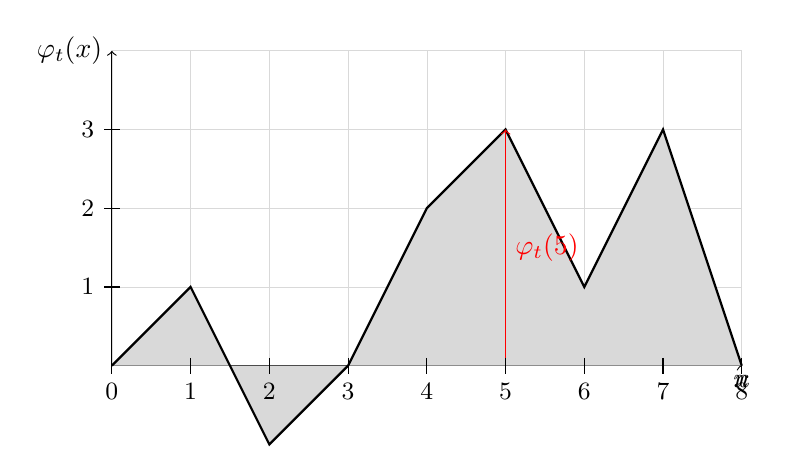
\begin{tikzpicture}
    % Define the coordinates of the fluctuating interface
    \draw[very thin,color=gray!30] (0,0) grid (8,4);
    \draw[<->] (0,4) node[left] {$\varphi_t(x)$} -- (0,0) -- (8,0) node[below] {$x$};

    % Define the vertices of the polygon
    \fill[gray!30] (0,0) 
        -- (1,1) 
        -- (2,-1) 
        -- (3,0) 
        -- (4,2) 
        -- (5,3) 
        -- (6,1) 
        -- (7,3) 
        -- (8,0) 
        -- cycle;

    % Draw the line of the fluctuating interface
    \draw[thick] (0,0) 
        -- (1,1) 
        -- (2,-1) 
        -- (3,0) 
        -- (4,2) 
        -- (5,3) 
        -- (6,1) 
        -- (7,3) 
        -- (8,0);

    % Draw the red arrow
    \draw[red,->] (5,0) -- (5,3) node[midway,right] {$\varphi_t(5)$};

    % Draw the x-axis labels
    \foreach \x in {0,1,2,3,4,5,6,7,8}
        \draw (\x,0.1) -- (\x,-0.1) node[below] {\small \x};

    % Draw the y-axis labels
    \foreach \y in {1,2,3}
        \draw (0.1,\y) -- (-0.1,\y) node[left] {\small \y};

    % Add labels for n
    \node[below] at (8,0) {$n$};
\end{tikzpicture}

\end{document}